\chapter{تعمیم آزمون چپمن-کولموگروف}
\label{ch3} 

\section{آزمون چپمن-کولموگروف برای دو فرایند وابسته}

برای تخمین طول مارکوف با استفاده از آزمون چپمن-کولموگروف ابتدا باید تعمیم معادله چپمن-کولموگروف \ref{ck_equation} برای دو فرایند وابسته را در نظر داشته باشیم.
\begin{equation}
  p(\vec{r}_{i+2}, \vec{r}_{i})=\int_{-\infty}^{+\infty} \mathrm{d} \vec{r}_{i+1} p(\vec{r}_{i+2} | \vec{r}_{i+1}) p(\vec{r}_{i+1}, \vec{r}_{i})
  \label{ck_equation_vec}
\end{equation}
مشابه رابطه \ref{chapmann_test} کمیت $S$ را نیز می‌توان به شکل زیر به دست آورد.
\begin{equation}
  S(\vec{r}_{i},t_{i}; \vec{r}_{j},t_{j} )=p(\vec{r}_{i}, t_{i} ; \vec{r}_{j}, t_{j})-\int_{-\infty}^{+\infty} \mathrm{d} \vec{r}_k p(\vec{r}_{i}, t_{i} | \vec{r}_k, t_k) p(\vec{r}_k, t_k ; \vec{r}_{j}, t_{j})
\end{equation}
در حالتی که چند فرایند وابسته داریم، هر یک از فرایندها می‌توانند نسبت به خودشان و یکدیگر طول‌های مارکوف‌ متفاوتی داشته باشند. بنابراین وقتی دو فرایند وابسته داریم ممکن است تا ۴ طول مارکوف متفاوت داشته باشیم، برای پیدا کردن این طول‌ها می‌توانیم روابط زیر را در نظر بگریم.
\begin{equation}
\begin{array}{l}
  {S_{1}(x_{i}, t_{i}; x_{j}, t_{j})=\int_{-\infty}^{+\infty} \mathrm{d} y_{i} \mathrm{d} y_{j} S_{i j}(\vec{r}_{i},t_{i}; \vec{r}_{j},t_{j} )} \\
  {S_{2}(x_{i}, t_{i}; y_{j}, t_{j})=\int_{-\infty}^{+\infty} \mathrm{d} y_{i} \mathrm{d} x_{j} S_{i j}(\vec{r}_{i},t_{i}; \vec{r}_{j},t_{j} )} \\
  {S_{3}(y_{i}, t_{i}; x_{j}, t_{j})=\int_{-\infty}^{+\infty} \mathrm{d} x_{i} \mathrm{d} y_{j} S_{i j}(\vec{r}_{i},t_{i}; \vec{r}_{j},t_{j} )} \\
  {S_{4}(y_{i}, t_{i}; y_{j}, t_{j})=\int_{-\infty}^{+\infty} \mathrm{d} x_{i} \mathrm{d} x_{j} S_{i j}(\vec{r}_{i},t_{i}; \vec{r}_{j},t_{j} )}\end{array}
\end{equation}
روابط بالا به ترتیب از بالا برای تخمین طول مارکوف فرایند $x$ نسبت به خودش، فرایند $x$ نسبت به $y$، فرایند $y$ نسبت به $x$ و فرایند $y$ نسبت به خودش استفاده می‌شوند. در نهایت از قدرمطلق روابط بالا انتگرال خواهیم گرفت.
\begin{equation}
\begin{aligned} 
  S_{1}(t_{i}, t_{j}) &=\int d x_{i} d x_{j}\left|S_{1}(x_{i}, t_{i}; x_{j}, t_{j})\right|, \quad \quad S_{1}(t_{i}, t_{j})=0 \Longrightarrow l_1=t_{i}-t_{j} \\
  S_{2}(t_{i}, t_{j}) &=\int d x_{i} d y_{j}\left|S_{2}(x_{i}, t_{i}; y_{j}, t_{j})\right|, \quad \quad S_{2}(t_{i}, t_{j})=0 \Longrightarrow l_2=t_{i}-t_{j}  \\
  S_{3}(t_{i}, t_{j}) &=\int d y_{i} d x_{j}\left|S_{3}(y_{i}, t_{i}; x_{j}, t_{j})\right|, \quad \quad S_{3}(t_{i}, t_{j})=0 \Longrightarrow l_3=t_{i}-t_{j} \\
  S_{4}(t_{i}, t_{j}) &=\int d y_{i} d y_{j}\left|S_{4}(y_{i}, t_{i}; y_{j}, t_{j})\right|, \quad \quad S_{4}(t_{i}, t_{j})=0 \Longrightarrow l_4=t_{i}-t_{j}  \end{aligned}
  \label{coupled_cktest}
\end{equation}
طول مارکوف فرایند $x$ نسبت به خودش با $l_1$ نشان داده می‌شود. طول‌های مارکوف دیگر نیز با $l_2$، $l_3$ و $l_4$ نشان داده می‌شوند.
در این حالت نیز می‌توانیم برای دو فرایند غیرمارکوف وابسته مانا آزمون چپمن-کولموگروف را بر حسب $\tau$ بنویسیم. 

تا اینجا آزمون چپمن-کولموگروف را برای دو فرایند غیرمارکوف وابسته تعمیم داده‌ایم، حال برای آزمایش این روش نیاز به 
مدلی داریم که بتواند سری‌های زمانی وابسته با طول مارکوف دلخواه تولید کند. در بخش بعدی با تعمیم مدل خودبرگشت 
مدل ساده‌ای را معرفی می‌کنیم که می‌توان طول مارکوف دو فرایند $x$ و $y$ را نسبت به خودشان و نسبت به 
یکدیگر در آن مشخص کرد.
% \FloatBarrier

\section{دو فرایند غیرمارکوف وابسته با طول مارکوف دلخواه}

\begin{figure}[H]
  \centering
  \subcaptionbox{فرایند $x$ با $l_1=20$، $l_2=10$.\label{fig:coupled_x}}
  {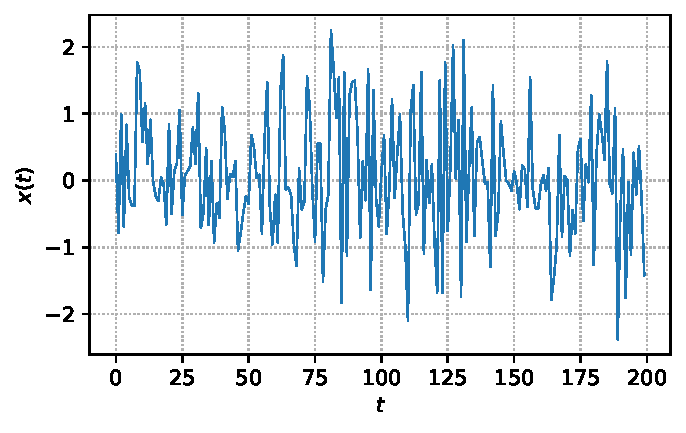
\includegraphics[width=0.49\textwidth]{images/toy_model_sample_0.pdf}}
  \subcaptionbox{فرایند $y$ با $l_3=15$، $l_4=25$.\label{fig:coupled_y}}
  {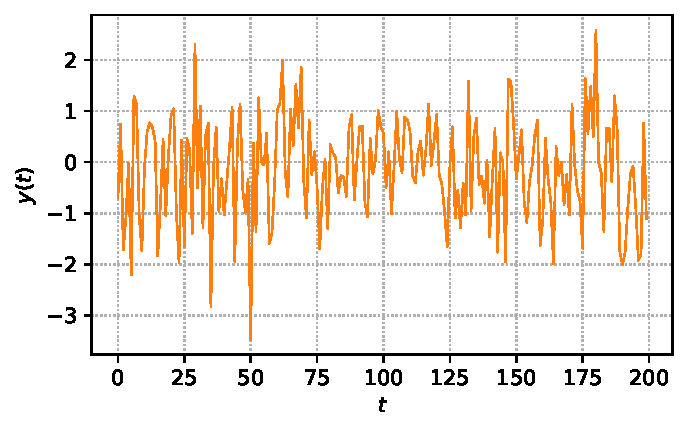
\includegraphics[width=0.49\textwidth]{images/toy_model_sample_1.pdf}}
  \caption{یک نمونه از فرایند $x$ و فرایند $y$ تولید شده با استفاده از \ref{coupledToymodel}.}\label{fig:coupled_xy}
\end{figure}
در مدل خودبرگشت \ref{ar_model} دیدیم که برای ساخت فرایند تصادفی با حافظه دلخواه حالت‌های گذشته $x$ در حالت بعدی $x$ به شکل مجموع آن‌ها دخالت داده شده‌اند.
برای ایجاد جفت‌شدگی بین دو فرایند تصادفی $x$ و $y$ نیز می‌توان حالت‌های گذشته هر یک از فرایندها را در دیگری دخالت دهیم. 
برای این کار مانند بخش قبل حالت‌های گذشته $y$ را به شکل وزن دار با رابطه \ref{ar_model} جمع می‌کنیم. فرایند دیگری هم 
مشابه $x$ با ضرایب مخصوص به خود برای $y$ می‌نویسیم. بنابراین داریم:
\begin{equation}
  \begin{array}{l}
    x_{t+1}=\sum_{n=1}^{l_1} \phi^{xx}_{n} x_{t-n}  + \sum_{n=1}^{l_2} \phi^{xy}_{n} y_{t-n} + \xi^{x}_{t} \\ \\
    y_{t+1}=\sum_{n=1}^{l_3} \phi^{yx}_{n} x_{t-n}  + \sum_{n=1}^{l_4} \phi^{yy}_{n} y_{t-n} + \xi^{y}_{t}
  \end{array}
  \label{coupledToymodel}
\end{equation}
در روابط \ref{coupledToymodel} چهار ضریب $\phi^{xx}_n$، $\phi^{xy}_n$، $\phi^{yx}_n$ و $\phi^{yy}_n$ ضرایب ثابتی هستند.
$\xi^x_t$ و $\xi^y_t$ هم نیروی‌های تصادفی گاوسی مستقل از هم هستند. $l_1$ و $l_2$ به ترتیب طول حافظه $x$ نسبت به خودش و $y$ را تعیین می‌کنند، به 
طور مشابه $l_3$ و $l_4$ نیز طول حافظه $y$ نسبت به فرایند $x$ و خودش را مشخص می‌کنند. 
در شکل \ref{fig:coupled_xy} بخشی از دو فرایند وابسته با $l_1=20$، $l_2=10$، $l_3=15$ و $l_4=25$ رسم شده است. 
در شکل \ref{fig:coupledXY} نیز دو فرایند $X(t)$ و $Y(t)$ رسم شده‌اند که به رابطه \ref{coupled_brownian} تعریف می‌شوند.

\begin{figure}[H]
  \centering
  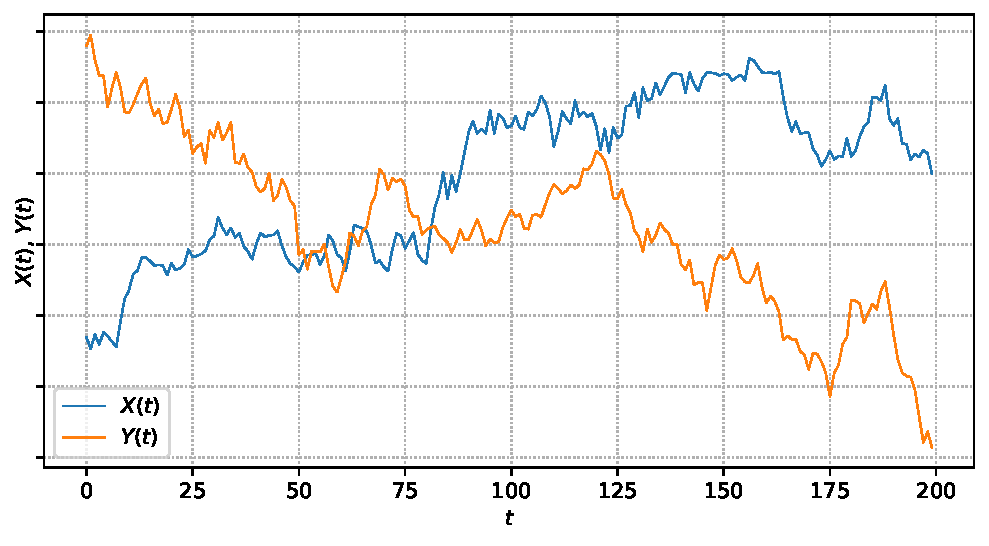
\includegraphics[width=\textwidth]{images/toy_model_sample_coup.pdf}
  \caption{در این شکل $X(t)$ و $Y(t)$ از رابطه \ref{coupled_brownian} محاسبه شده است.}\label{fig:coupledXY}
\end{figure}

\begin{equation}
  \begin{array}{l}
    X(t+\tau)=X(t)+\tau x(t) \\ Y(t+\tau)=Y(t)+\tau y(t)
    \label{coupled_brownian}
  \end{array}
\end{equation}
در حالتی که فقط یک نمونه از فرایند $x$ و $y$ را داشته باشیم، مثل حالت قبل فقط می‌توانیم $S$ را بر حسب $\tau$ به دست بیاوریم. 
با این تفاوت که برای دو فرایند وابسته باید $S_{1}(\tau)$، $S_{2}(\tau)$، $S_{3}(\tau)$ و $S_{4}(\tau)$ را محاسبه کنیم.
در شکل \ref{fig:singleCCKtestxx} وابستگی فرایند $x$ به خودش با $S_{1}(\tau)$ و در شکل \ref{fig:singleCCKtestxy} 
وابستگی فرایند $x$ به $y$ با $S_{2}(\tau)$ نشان داده شده است. در شکل \ref{fig:singleCCKtestxx} مقدار $S_{1}(\tau)$ 
در $\tau = 21$ با در نظر گرفتن خطا صفر شده است که نشان دهنده این است که $l_1 = 20$ است و این مقدار به درستی تخمین زده شده است.
در شکل \ref{fig:singleCCKtestxy} نیز با در نظر گرفتن خطا $S_{2}(\tau)$ در $\tau=11$ صفر شده است که نشان دهنده تخمین درست 
برای $l_2=10$ است. به طور مشابه در شکل \ref{fig:singleCCKtestyx} نشان دهنده وابستگی فرایند $y$ به فرایند $x$ است که $S_{3}(\tau)$ با در نظر گرفتن خطا 
در $\tau = 16$ صفر شده است که نشان دهنده این است که $l_3 = 15$ است. در شکل \ref{fig:singleCCKtestyy} نیز $S_{4}(\tau)$ 
در $\tau=26$ با در نظر گرفتن خطا صفر شده است که نشان دهنده این است که $l_4 = 25$ است.

\begin{figure}[H]
  \centering
  \subcaptionbox{$S_{1}(\tau)$ که نشان‌دهنده وابستگی فرایند $x$ به خودش است در $\tau = 21$ با در نظر گرفتن خطا صفر شده است.\label{fig:singleCCKtestxx}}
  {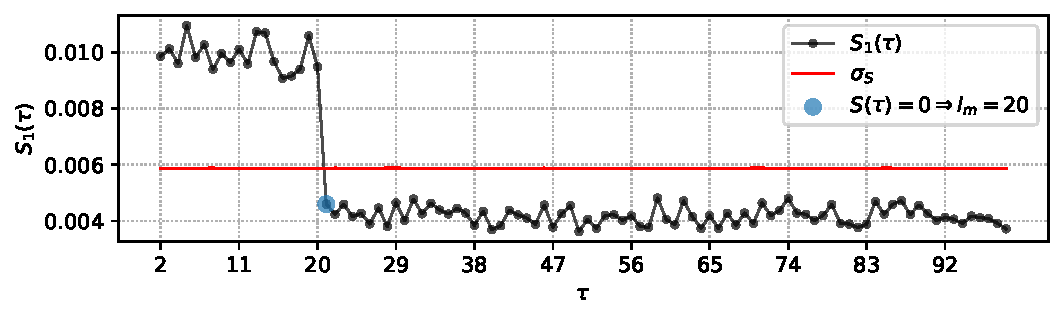
\includegraphics[width=0.9\textwidth]{images/singleCCKtestxx.pdf}}
  \subcaptionbox{$S_{2}(\tau)$ که نشان‌دهنده وابستگی فرایند $x$ به $y$ است در $\tau = 11$ با در نظر گرفتن خطا صفر شده است.\label{fig:singleCCKtestxy}}
  {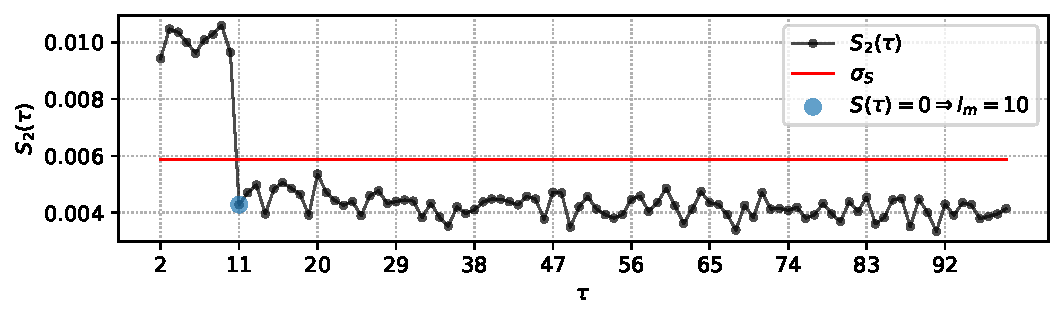
\includegraphics[width=0.9\textwidth]{images/singleCCKtestxy.pdf}}
  \caption{نمودار $S_{1}(\tau)$ و $S_{2}(\tau)$ که نشان دهنده وابستگی فرایند $x$ به خودش و به فرایند $y$ هستند.}\label{fig:singleCCKtestx}
\end{figure}
% \FloatBarrier
\begin{figure}[H]
  \centering
  \subcaptionbox{$S_{3}(\tau)$ که نشان‌دهنده وابستگی فرایند $y$ به فرایند $x$ است در $\tau = 16$ با در نظر گرفتن خطا صفر شده است.\label{fig:singleCCKtestyy}}
  {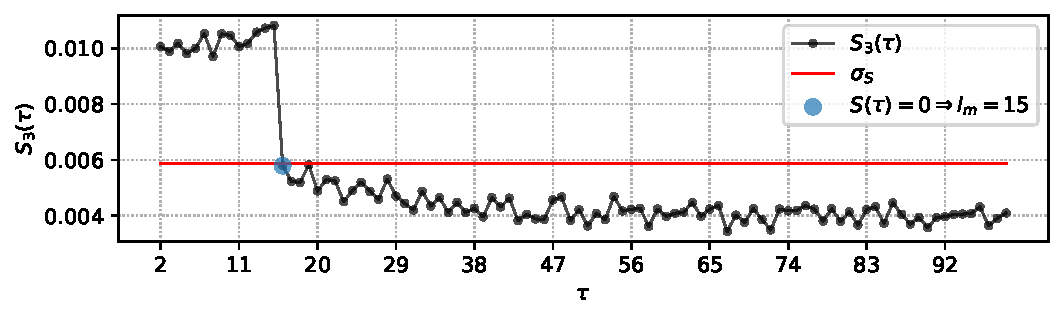
\includegraphics[width=0.9\textwidth]{images/singleCCKtestyx.pdf}}
  \subcaptionbox{$S_{4}(\tau)$ که نشان‌دهنده وابستگی فرایند $y$ به خودش است در $\tau = 26$ با در نظر گرفتن خطا صفر شده است.\label{fig:singleCCKtestyx}}
  {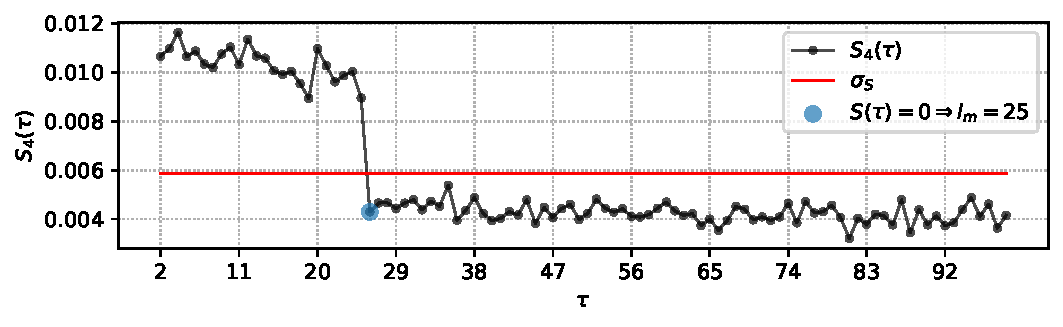
\includegraphics[width=0.9\textwidth]{images/singleCCKtestyy.pdf}}
  \caption{نمودار $S_{3}(\tau)$ و $S_{4}(\tau)$ که نشان دهنده وابستگی فرایند $y$ به فرایند $x$ و به خودش هستند.}\label{fig:singleCCKtesty}
\end{figure}

\begin{figure}[H]
  \centering
  \subcaptionbox{$S_1( t_i, t_i - 13) = 0$, $l_1=12$\label{fig:CCKtestxx}}
  {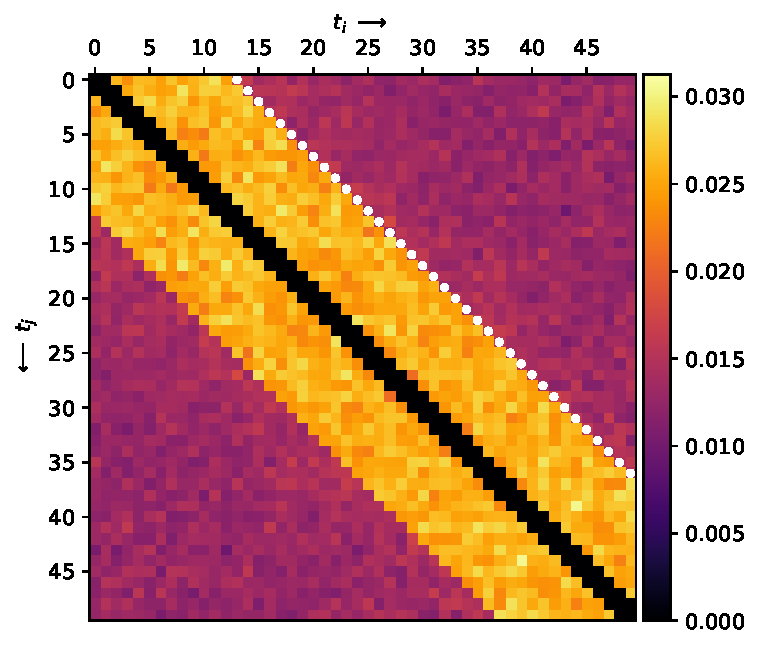
\includegraphics[width=0.49\textwidth]{images/CCKtestxx.pdf}}
  \subcaptionbox{$S_2( t_i, t_i - 7 ) = 0$, $l_2=6$\label{fig:CCKtestxy}}
  {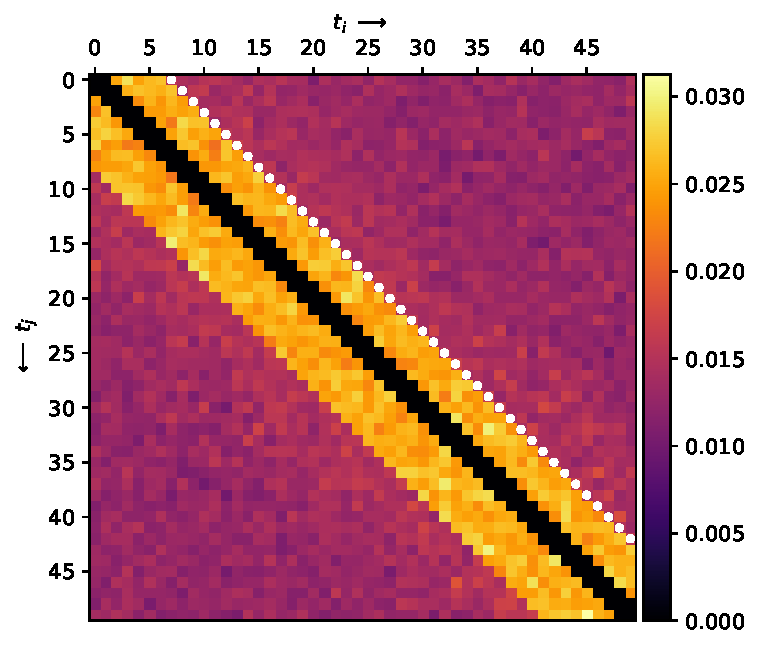
\includegraphics[width=0.49\textwidth]{images/CCKtestxy.pdf}}
  \caption{نمودار $S_{1}( t_i, t_j )$ و $S_{2}( t_i, t_j )$ که نشان دهنده وابستگی فرایند $x$ به خودش و به فرایند $y$ هستند.}\label{fig:CCKtestx}
\end{figure}
در قدم بعدی آزمون چپمن-کولموگروف را برای بیشتر از یک نمونه از فرایند $x$ و $y$ به کار خواهیم برد. برای این کار $3 \times 10^5$ 
نمونه برای هر یک از فرایندهای $x$ و $y$ تولید شده است.
طول مارکوف برای این دو فرایند به شکل زیر تعیین شده است.
\begin{equation}
  \begin{array}{l}
    l_1 = 12, l_2 = 6 \\
    l_3 = 8, l_4 = 10
  \end{array}
  \label{ctoymodell}
\end{equation}
مانند حالتی که یک فرایند داشتیم در اینجا نیز می‌توانیم ماتریس $S(t_i, t_j)$ را به دست بیاوریم که در واقع 
شامل چهار ماتریس $S_1$، $S_2$، $S_3$ و $S_4$ می‌شود.
 شکل \ref{fig:CCKtestx} و \ref{fig:CCKtesty} نتیاج آزمون چپمن-کولموگروف برای دو فرایند $x$ و $y$ 
 در این تصاویر هم نقاط سفید رنگ نشان دهنده جایی است که $S$ با در 
 نظر گرفتن خطا صفر شده است.
 شکل \ref{fig:CCKtestxx} نمایش گرافیکی ماتریس $S_1$ است که 
 همانطور که از شکل پیداست $S_1( t_i, t_i - 13) = 0$ که نشان دهنده 
 تخمین درست $l_1 = 12$ است. شکل \ref{fig:CCKtestxy} نیز نمایش گرافیکی ماتریس $S_2$ است 
 که $S_2( t_i, t_j ) $ به ازای $t_i \geq t_j + 7$ برابر با صفر است که نشان دهنده این است که 
 $l_2 = 6$ است. به طور مشابه در شکل \ref{fig:CCKtestyx} و \ref{fig:CCKtestyy} ماتریس‌های $S_3$ و $S_4$ 
 به شکل گرافیکی ترسیم شده‌اند. همانطور که پیداست $S_3( t_i, t_j )$ به ازای $t_i \geq t_j + 9$ و 
$S_4( t_i, t_j )$ به ازای $t_i \geq tـj + 11$ با در نظر گرفتن خطا صفر شده‌اند که نشان‌دهنده 
این است که $l_3 = 8$ و $l_4 = 10$ است که همان مقادیر اولیه \ref{ctoymodell} هستند.
 
\begin{figure}[H]
    \centering
    % \vspace{1cm}
    \subcaptionbox{$S_3( t_i, t_i - 9) = 0$, $l_3=8$\label{fig:CCKtestyx}}
    {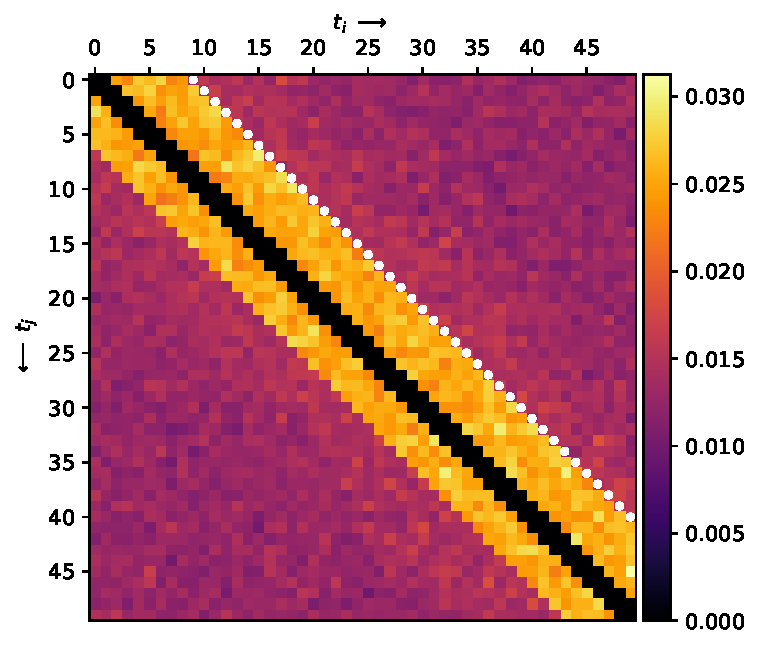
\includegraphics[width=0.49\textwidth]{images/CCKtestyx.pdf}}
    \subcaptionbox{$S_4( t_i, t_i - 11) = 0$, $l_4=10$\label{fig:CCKtestyy}}
    {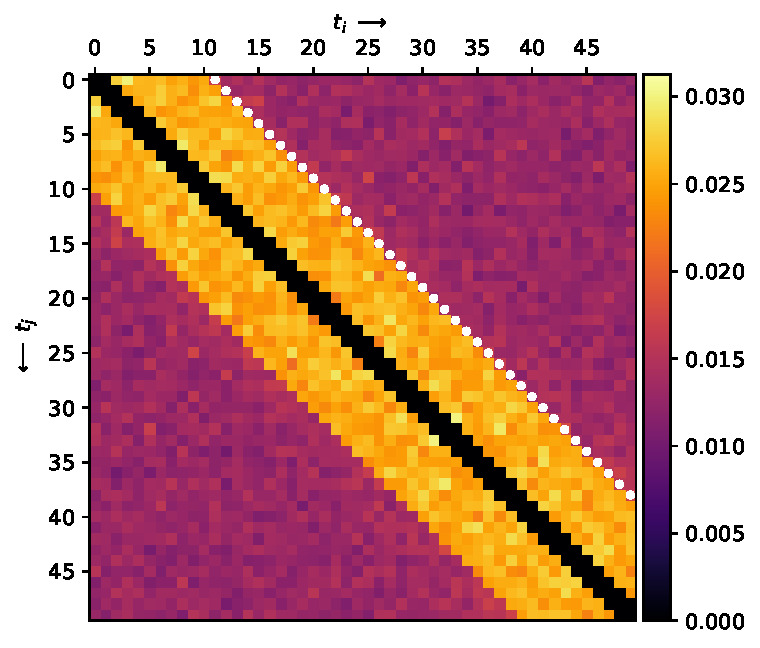
\includegraphics[width=0.49\textwidth]{images/CCKtestyy.pdf}}
    \caption{نمودار $S_{3}( t_i, t_j )$ و $S_{4}( t_i, t_j )$ که نشان دهنده وابستگی فرایند $y$ به فرایند $x$ و به خودش هستند.}\label{fig:CCKtesty}
\end{figure}
تا اینجا آزمون چپمن-کولموگروف را برای دو فرایند غیرمارکوف وابسته تعمیم داده‌ایم و همچنین با تعمیم مدل خودبرگشت به 
دو فرایند، آزمون چپمن-کولموگروف تعمیم یافته را روی سری‌های زمانی تولید شده با این مدل آزمایش کردیم. در فصل بعد 
از آزمون چپمن-کولموگروف تعمیم یافته برای محاسبه طول مارکوف سری‌های زمانی مالی\LTRfootnote{Financial time series} استفاده خواهیم کرد.
